\chapter{Project Plan and Methodology}

The project methodology is summarised in \cref{fig:project-plan-methodology}. 

Further analysis of the necessary modelling, simulation and design elements are presented.

A plan is presented for experimentation to both verify design choices and answer research questions.

\section{Modelling, Simulation \& Design}

The geometric design of the leg, having already been chosen, will be further developed in theory and kinematic workspace simulations will be performed to confirm the leg linkage lengths for optimal performance. The kinematic mappings of the leg will be developed as the final step in leg design.

A virtual compliance model needs to be developed to achieve: launch energy control, impact energy control, and steady state performance. First the low level spring-damper mass motion will be considered, deriving the necessary equations to design a suitable virtual compliance model.

Both the dynamic and kinematic models will be simulated and iteratively corrected if necessary.

The design of the leg will be split into hardware and software elements - where hardware includes mechanical and electrical design, and software includes embedded system and GUI design. Throughout the hardware design of the leg each element will be critically considered by modelling, iterative design, and theoretical design, as the case dictates. 

A kinematic workspace model will be developed to present predictions of current usage, motor torques, and end effector forces - this will help validate hardware and software design choices with the research questions in mind.

The software design will be developed after the hardware design is at a usable level. This will enable testing of the system as it is developed and addition of necessary functions. The core of the software development will involve the design of a communication system for all elements of the electrical hardware design.

A controller will be developed through theory and simulation, before being implemented and tested in experimentation. This will be an iterative process where hardware, software, and the underlying control system will be adapted to meet the necessary specifications.

\section{Testing \& Verification}

The aim of this project is to develop a robust robotic platform capable of performing high acceleration jumps using a virtual model - the experiments conducted will reflect that and develop the control system to such a point that it meets these design specifications. 

At each stage of experimentation the scientific method will be introduced, where aims of the experiment are outlined, before the experimental data is analysed and a summary is presented clarifying whether the aims have been met. Verification of the experiments will result from comparison of the experimental data to previous simulated and theoretical data as well as critical analysis.

Data will be logged including control system data, virtual model forces, motor signals and kinematic positions. Along with this data all experiments will be recorded for later analysis. The leg will be mounted on the robotic guide platform.

Tests will be performed to investigate various virtual model spring-damper topologies, and the fidelity of the response achieved. These experiments will be presented as a comparison between practical data and theoretical design. If the theoretical design is not shown in the practical data then the necessary steps will be taken to correct that if possible - this is the iterative design component of the experiment. 

Drop tests will be performed to determine the best virtual model configuration for leg impact, and to investigate the robustness of the leg design.

The spring-damper tests will inform the configuration of the virtual model for jump tests, where the spring-damper constants will be chosen from experimental analysis. The jump tests will investigate all phases of jumping individually. 

The design specifications say the leg needs to be robust. In order to test this an experiment will be performed to determine the repeatability of jumps, investigating force control fidelity and disturbance rejection.

The motor and motor driver combination will be experimentally tested for correct operation - in the form of response time, set-point tracking, and steady state error.

The final phase of experimentation will be to perform basic trajectory tracking. This will test kinematic fidelity and dynamic performance likely to be experienced in further legged locomotion study.

\begin{figure}[]
\centering
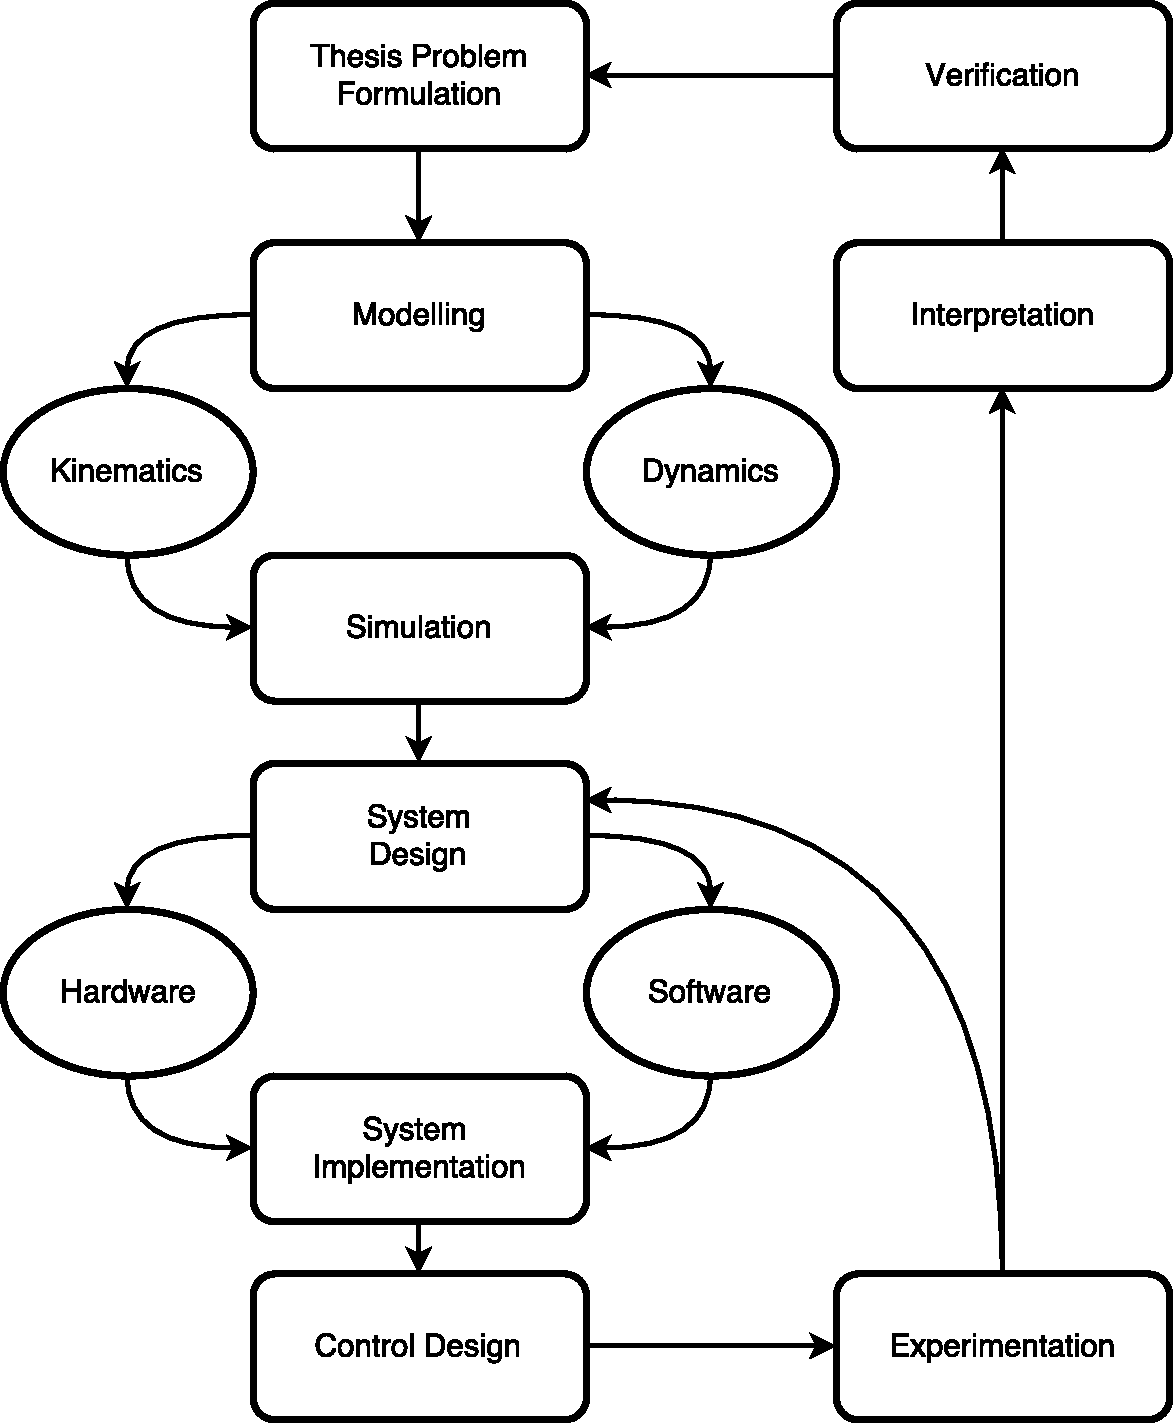
\includegraphics[width=0.8\textwidth]{images/introduction/project-plan-methodology.pdf} 
\caption{Baleka thesis project methodology flow chart.}
\label{fig:project-plan-methodology}
\end{figure}
